\documentclass[conference]{IEEEconf}
%\documentclass[sigconf]{acmart}
\usepackage{cite}
\usepackage{amsmath,amssymb,amsfonts}
\usepackage{algorithmic}
\usepackage{graphicx}
\usepackage{textcomp}
\usepackage{xcolor}
%\usepackage{latex8}
%\usepackage{times}
%\pagestyle{empty}
\usepackage{epsfig}
\def\BibTeX{{\rm B\kern-.05em{\sc i\kern-.025em b}\kern-.08em
    T\kern-.1667em\lower.7ex\hbox{E}\kern-.125emX}}
    
\bibliographystyle{IEEEtran}
\graphicspath{./imaages/}

\newcommand{\mq}{\mbox{\em MQ}}

\title{ 
        	Cloud Native Software Engineering Research Landscape
      }


\author{
			Brian Mitchell\\
			College of Computing and Informatics\\
			Drexel University, Philadelphia, PA, USA\\
			bmitchell@drexel.edu
} 

\date{}

\begin{document}

%\bibliographystyle{latex8}

\maketitle

\thispagestyle{empty}


\begin{abstract}
Since the mid 2010's we have seen significant shifting of traditional brick-and-mortar businesses in adopting public cloud infrastructure.  Early skepticism about moving strategic business to the cloud on based on security or technical risk have been replaced with aggressive plans to migrate that is well supported by both technical professionals and senior management. In fact, IDC estimates that the overall worldwide cloud spend will almost double from \$706.6B in 2021 to \$1.3T by 2025\cite{IDCReport}.  

It seems while everybody is embracing the cloud computing model, little attention has been paid to ways that mature software engineering practices needed to move to this new computing model at scale. Early successes by technology startups, or by industry moving their existing suite of web and mobile services over to the cloud are now being followed with ambitious plans to move more of their core business to the cloud, and to innovate new products and services that could only be delivered in the cloud.

While there is a significant research activity in many areas of cloud computing, little attention has been paid to the needs of the software engineering professional.  This paper will focus on the landscape of Cloud Native Software Engineering from a practitioners standpoint, and attempt to identify some research opportunities in this space.
\end{abstract}  

\section{Introduction}
\label{Intro}
Delivering managed computing services via hosted infrastructure stared in the late 1990's with the introduction of the Software as a Service (SaaS) model. One of the earliest examples of this new model is Salesforce.com, that launched in 1999\cite{SalesforceHistory}.  Salesforce offered a best-in-class customer relationship management (CRM) suite, but its software was not as disruptive as its delivery model. Unlike other competitors that licensed you software that you ran on your own equipment, Salesforce pioneered the pay-as-you-go SaaS subscription model. In this model, you simply pay a monthly per-user charge and can access the solution from any device at any time.     

While SaaS solutions , cloud computing as we know it today can be attributed to the launch of AWS (Amazon) \cite{AWSLaunch} in early 2006, with Azure (Microsoft)\cite{AzureLaunch} and GCP (Google)\cite{GCPLaunch} following in 2008. Early adopters of cloud infrastructure were largely technology companies that innovated patterns, practices, and open sourced many tools and frameworks to highlight the benefits of running resilient and scalable business services in the public cloud.  


\section{What is Cloud Native Computing?}
\label{sec:WhatIsCNF}
Before we explore the software engineering landscape for the cloud, we need to address exactly what we mean by cloud native computing.  According to the Cloud Native Computing Foundation (CNCF)\cite{CNCFHome}  \textit{"Cloud native technologies empower organizations to build and run scalable applications in modern, dynamic environments such as public, private, and hybrid clouds."}.  Amazon's definition is \textit{"Cloud native technologies empower organizations to build and run scalable applications in modern, dynamic environments such as public, private, and hybrid clouds"}. Google offers the definition \textit{"Cloud native means adapting to the many new possibilities—but very different set of architectural constraints—offered by the cloud compared to traditional on-premises infrastructure."}.  The primary theme in these definitions centers around the role that technologies play in enabling the creation of cloud native applications.

We think a better definition of cloud native computing that focuses more on  software engineering is \textit{"Cloud native applications are well architected systems, that are "container" packaged, and dynamically managed"}. Specifically:

\begin{itemize}
	\item \textbf{Well Architected Systems} - By this we mean systems that adhere not only to established software engineering best practices but also embrace specific functional and non-functional capabilities offered by the cloud. For example, how are the computing components identified, how are they work with each other, how are security requirements met, how is the system designed for resiliency and scale?
	
	\item  \textbf{Container Packaged} - The term \textit{container} is overloaded in the cloud computing terminology landscape.  In many places its equated to a standardized package that is managed by Docker\cite{DockerContainer} technologies - aka "a docker container".  We take a more generic view of container packaging. Specifically, we think container packaging is a mechanism to package and deploy code that is ephemeral, can operate across a variety of different hardware architectures (e.g., Intel, ARM, etc), and at runtime is supervised.  Supervision includes full lifecycle management associated with version identification, startup, shutdown, health checks, and monitoring.  Examples of container packaging and supervision include Docker, Docker Compose, Kubernetes, and serverless \cite{baldini2017serverless}. We also include in this category the emerging popularity of using server-side web assembly\cite{haas2017bringing, bosshard2020use} as a way to package and deploy cloud native application services. 

	\item \textbf{Dynamically Managed} - One interesting conceptual model for cloud computing is to consider the cloud as a large, highly distributed, special purpose operating system. Just like any operating system, there are a number of resource types that need to be provided to applications like storage, compute, network and security services.  The job of an operating system is to dynamically manage and optimize the allocation of these resources to the realtime computing demand.  When done well, every process being managed by the OS will perceive that it has access to the resources it needs, when it needs it.  In a similiar context, a cloud service provider can be 
	
	
	\item 
	 
\end{itemize} 


b
v
v
v
v

v
vv

v
vv
vv
v

v
vv
vv
vvv
v

v
vv


v


v

vv

vv
vv



\begin{figure*}[t!]
	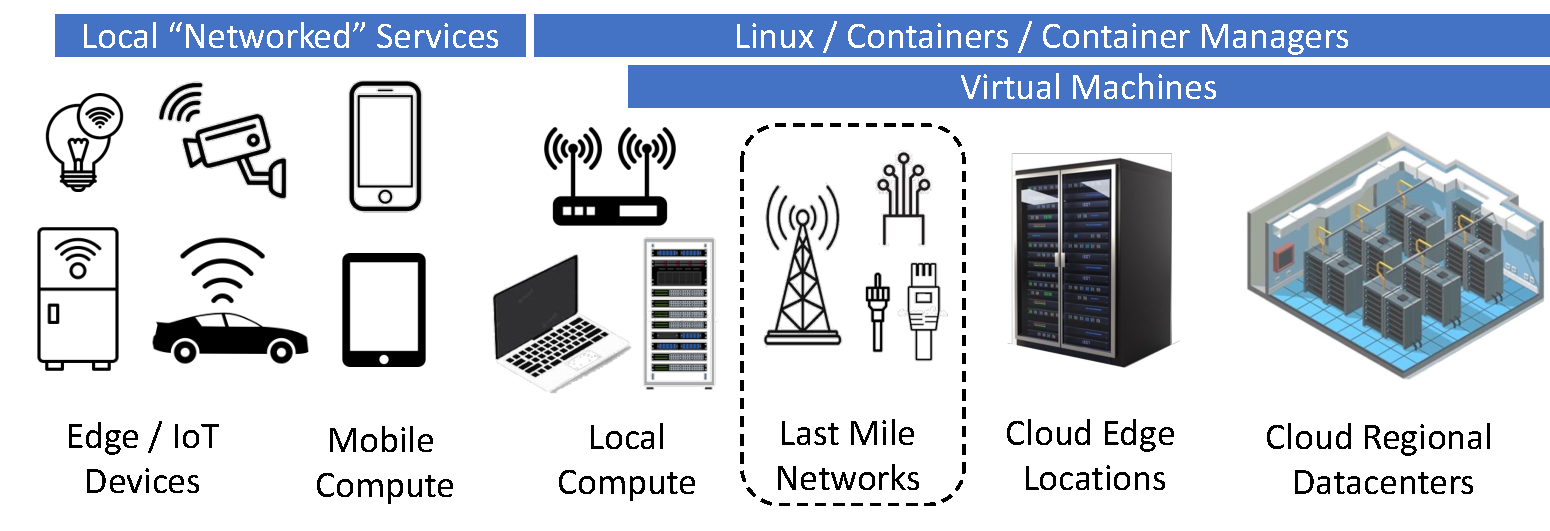
\includegraphics[width=\textwidth]{images/CloudTopo2.pdf}	
	\caption{Cloud Compute - From Big to Small}
\end{figure*}

\section{Software Architecture Requirements}
\label{sec:SoftwareArchitecture}

\section{Software Construction Requirements}
\label{sec:SoftwareConstruction}

\subsection{Polyglot Programming}
\label{subsec:Polyglot}



\bibliography{CloudNative.bib}
\end{document} 